%#######################################################################################
%############################		CABECERA		####################################
%#######################################################################################
\documentclass[a4,12pt,onecolum]{article}
\usepackage[utf8]{inputenc}
\usepackage[spanish]{babel} 		% para que divida bien las silabas en final de linea
\usepackage[margin=3cm]{geometry}	% para poner los margenes bonitos
\usepackage{fancyhdr}
\usepackage{graphicx} 				% meter figuras gráficas
\graphicspath{{fotos/}}
\usepackage{import}
\usepackage{color} 					% para introducir colores en el documento
\usepackage{verbatim}
\usepackage{subfigure}
\usepackage{listings}
\usepackage{cite}
%\bibliographystyle{alpha}
\usepackage[official]{eurosym}
\usepackage{graphicx}
\usepackage{fancyhdr}
\usepackage{subfigure}
\usepackage{listings, courier}
\usepackage{amssymb, amsmath, amsbsy}
\usepackage{float}
\usepackage[colorinlistoftodos]{todonotes}
\usepackage{cite}
\PassOptionsToPackage{hyphens}{url}\usepackage{hyperref}
\usepackage{url, hyperref}
\usepackage[nottoc]{tocbibind}
\usepackage{titlesec}
\usepackage{fancyvrb}
\setlength{\headheight}{20pt}


% FIGURAS [htbp] significa que el orden para que LaTeX trate de incrustar la imagen es: primero que lo intente aquí (h), luego en la parte de arriba (t), a continuación, en la parte de abajo (b), y por último, en la parte de arriba de la siguiente página (p). Puedes reordenar estas letras para seleccionar el orden que prefieras. Eso sí, muchas veces LaTeX hace lo que quiere. Pero si pones [htbp], indicas a LaTeX que ponga la imagen exactamente ahí. Para usar [htbp] tienes que cargar el paquete {float}.


%\usepackage{times} 						% tipo de letra periodico
%\renewcommand{\familydefault}{\sfdefault}	% tipo de letra Arial

% este bloque es para definir el estilo del texto C++
\lstset{language=C++,
  inputencoding=latin1,	% permite las tildes en el código
  backgroundcolor=\color[gray]{0.9},% color del fondo
  frame=single,		% dibuja un borde
  columns=flexible,	% el tamaño de letra se ajusta al ancho
  extendedchars=false,
  aboveskip=1eM,
  basicstyle=\ttfamily,
  keywordstyle=\color{blue}\ttfamily,
  stringstyle=\color{red}\ttfamily,
  commentstyle=\color{green}\ttfamily,
  morecomment=[l][\color{magenta}]{\#}
}

\hypersetup{
    bookmarks=true,         % show bookmarks bar?
    unicode=false,          % non-Latin characters IN Acrobat’s bookmarks
    pdftoolbar=true,        % show Acrobat’s toolbar?
    pdfmenubar=true,        % show Acrobat’s menu?
    pdffitwindow=false,     % window fit to page when opened
    pdfstartview={FitH},    % fits the width of the page to the window
    pdftitle={My title},    % title
    pdfauthor={Author},     % author
    pdfsubject={Subject},   % subject of the document
    pdfcreator={Creator},   % creator of the document
    pdfproducer={Producer}, % producer of the document
    pdfkeywords={keyword1} {key2} {key3}, % list of keywords
    pdfnewwindow=true,      % links IN new PDF window
    colorlinks=true,        % false: boxed links; true: colored links
    linkcolor=black,          % color of internal links (change box color with linkbordercolor)
    citecolor=blue,        % color of links to bibliography
    filecolor=magenta,      % color of file links
    urlcolor=blue           % color of external links
}

%\usepackage[hidelinks]{hyperref}% para anadir enlace dentro del documento, tiene que ser la ultima declaracion porque sino puede fallar

\title{Seguridad}
\date{\today}

%---------------------- ENCABEZADO Y PIE DE PÁGINA

\pagestyle{fancy}

\lhead{Seguridad}
\rhead{\leftmark}
\cfoot{\thepage}

\renewcommand{\headrulewidth}{0.4pt} % grosor de la línea de la cabecera
\renewcommand{\footrulewidth}{0.4pt} % grosor de la línea del pie


\setcounter{secnumdepth}{4}
\titleformat{\paragraph}
{\normalfont\normalsize\bfseries}{\theparagraph}{1em}{}
\titlespacing*{\paragraph}
{0pt}{3.25ex plus 1ex minus .2ex}{1.5ex plus .2ex}
%#######################################################################################
%##############################			CUERPO			################################
%#######################################################################################
\begin{document}

%################## PORTADA

\begin{titlepage}

\newcommand{\HRule}{\rule{\linewidth}{0.5mm}} % Defines a new command for the horizontal lines, change thickness here

\center % Center everything on the page

\textsc{\LARGE Universidad de Murcia}\\[0.8cm]
\textsc{\Large Grado en Ingeniería Informática}\\[0.5cm]
\textsc{\large 4º curso}\\[0.4cm]
\textsc{\large Grupo 6}\\[0.4cm]
\textsc{\large Curso 2016/2017 - Junio}\\[0.4cm]

\HRule \\[0.6cm]
{ \huge \bfseries Seguridad}\\[0.3cm]
\HRule \\[0.5cm]
{ \Large \bfseries Práctica final}\\[0.3cm]
\HRule \\[1.0cm]

%################## AUTORES

\begin{minipage}{0.4\textwidth}
\begin{flushleft} \large
Alumnos:\\
Cristian Roche Borja \\
\small{DNI: 76581531H}	\\
\large{Alicia Ruiz Tovar} \\
\small{DNI: 48693813F}
\end{flushleft}
\end{minipage}
~
\begin{minipage}{0.4\textwidth}
\begin{flushright} \large
Docentes: \\
Alberto Huertas Celdrán
Gabriel López Millán
Gregorio Martínez Pérez
\end{flushright}
\end{minipage}\\[1cm]

%################## LOGO

\centering

\includegraphics[width=0.5\textwidth]{./portada/logoum.png}\\[0.8cm] % Include a department/university logo - this will require the graphicx package

\end{titlepage}

%################## PAGINA EN BLANCO

\thispagestyle{empty}
\textcolor[rgb]{1.00,1.00,1.00}{palabra} % Pinta "palabra" de blanco
\newpage

\setcounter{page}{3}

%##################	TABLA DE CONTENIDOS

\newpage
\tableofcontents 		% indice
\rhead[\thepage]{Índice}
\newpage

%##################	CUERPO DEL DOCUMENTO

%################## INTRODUCCIÓN

%\section{Introducción}
%\rhead[\thepage]{\thesection. Introducción}

% #######################   OAUTH   ##################################

\clearpage
\section{Oauth}
\rhead[\thepage]{\thesection. Oauth}





% #######################   NMAP y Metasploit   ##################################

\clearpage
\section{NMAP y Metasploit}
\rhead[\thepage]{\thesection. NMAP y Metasploit}

\subsection{Víctima}
Utilizaremos una máquina virtual de prueba. Esta máquina ha sido creada con vulnerabilidades para la práctica de ataques. La URL de descarga es la \href{wiki.inf.um.es/metasploitable2/metasploitable-linux-2.0.0.zip}{siguiente}. \\

La IP de esta máquina es la \texttt{192.168.62.189}.

\subsection{Atacante}

\subsubsection{NMAP}

El equipo que actuará como atacante hace uso de la herramienta NMAP. Para instalarla ejecutamos el siguiente comando:

\begin{verbatim}
$ sudo apt-get install namp
\end{verbatim}

Establecemos en el archivo \emph{/etc/hosts}, equivalente al DNS local, la IP de la víctima (\texttt{192.168.62.189}) y la denominamos \texttt{metasploitable}, como muestra la figura \ref{fig:nmap1}. \\

\begin{figure}[htbp]
\centering
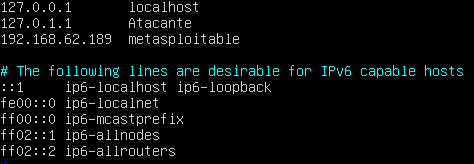
\includegraphics[width=0.5\textwidth]{./images/Atacante_dns_victima.png}
\caption{Atacante\_dns\_victima.}
\label{fig:nmap1}
\end{figure}

De esta forma, tenemos dos opciones para hacer referencia a la víctima. En la figura \ref{fig:nmap2} se observa el resultado de este escaneo simple fruto de cualquiera de estas dos opciones.

\begin{verbatim}
$ nmap 192.168.62.189
$ nmap metasploitable
\end{verbatim}

\begin{figure}[htbp]
\centering
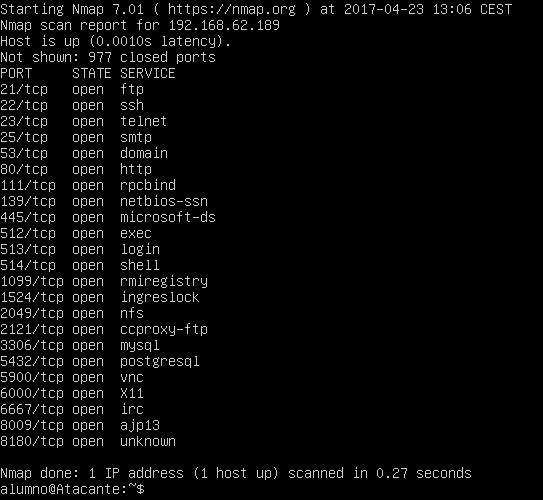
\includegraphics[width=0.8\textwidth]{./images/Atacante_nmap_simplescan.png}
\caption{Atacante\_nmap\_simplescan.}
\label{fig:nmap2}
\end{figure}

De forma un poco más elaborada, se puede ejecutar el escaneo de puertos haciendo uso de otras técnicas:

\begin{itemize}
  \item Mediante listado de equipos: \texttt{\$ nmap 192.168.62.1 192.168.62.10 192.168.62.189}
  \item Mediante subred: \$ nmap 192.168.62.0/24
  \item Mediante un fichero que almacene las IPs (o las expresiones de las mismas) a analizar: \$ nmap -iL hosts.txt, como muestra la figura \ref{fig:nmap3}.
\end{itemize}

\begin{figure}[htbp]
\centering
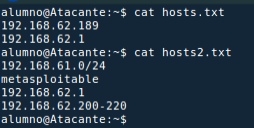
\includegraphics[width=0.4\textwidth]{./images/Atacante_nmapscan_filecomplex.png}
\caption{Atacante\_nmapscan\_filecomplex.}
\label{fig:nmap3}
\end{figure}

\subsubsection{NMAP con Metasploit}

También hemos de instalar Mestasploit para hacer uso de él: \url{https://github.com/rapid7/metasploit-framework/wiki/Nightly-Installers}. Una vez instalado, con \texttt{\$ msfconsole} inicializamos Metasploit y la base de datos asociada. \\

A continuación, realizamos un scanner básico de la red, almacenando el contenido en la base de datos interna y exportándolo completo de la misma a un fichero, para así analizarlo:

\begin{verbatim}
$ db_nmap -v -sV 192.168.62.0/24
$ db_export out_ejercicio1.txt
\end{verbatim}

Como muestra la figura \ref{fig:nmap4}, se observa que en dicho fichero encontramos el contenido del escaneo. Por un lado, podemos ver información del usuario que ha invocado el Metasploit. Seguidamente, tenemos el apartado que refiere a los hosts y servicios que se han encontrado en la dirección de subred que se le ha pasado al escaneo. Por último, podemos observar que el grueso del fichero son los módulos del Metasploit.

\begin{figure}[htbp]
\centering
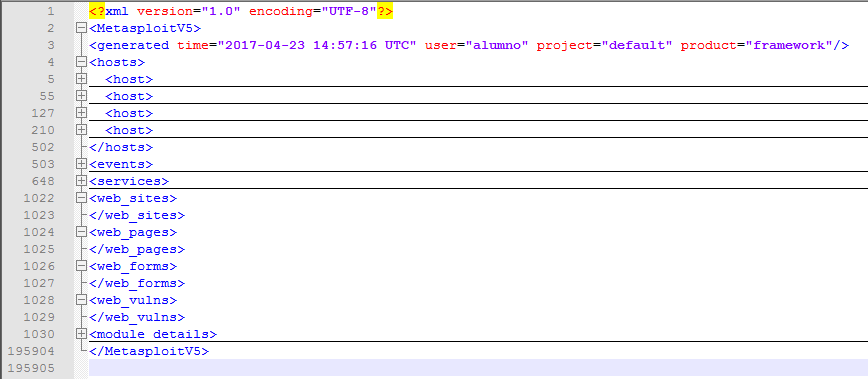
\includegraphics[width=1.0\textwidth]{./images/Atacante_scaner_y_BBDD.png}
\caption{Atacante\_scaner\_y\_BBDD.}
\label{fig:nmap4}
\end{figure}

% #######################   Wireshak: trazas   ##################################

\subsubsection{Wireshak: trazas}

A continuación mostramos algunas trazas obtenidas tras ejecutar ciertos comandos con NMAP.

\begin{itemize}
  \item \texttt{\$ nmap —scan-delay 1000ms -p 20-30 metasploitable}. En el host \texttt{metasploitable} se lanza un escaneo de puertos cada segundo a un puerto diferente entre los puertos 20 al 30, como muestra la figura \ref{fig:nmap5}. El fin principal de realizar un escaneo de puertos de esta forma es evitar ser detectado por la seguridad que pueda tener la subred.

  \begin{figure}[htbp]
  \centering
  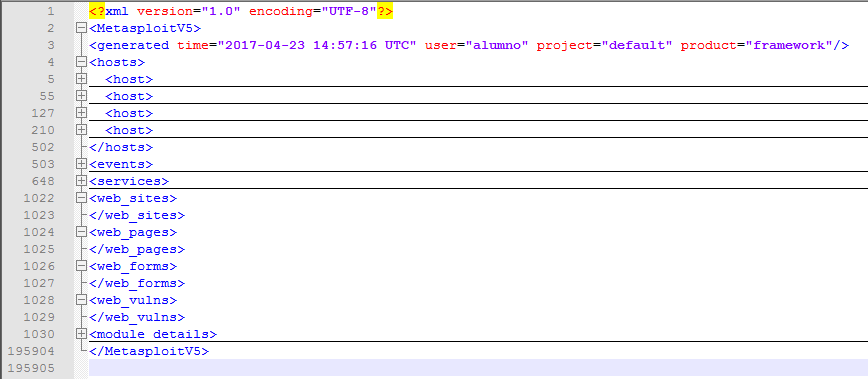
\includegraphics[width=1.0\textwidth]{./images/Atacante_scaner_y_BBDD.png}
  \caption{Atacante\_wireshar\_scaneo\_delay.}
  \label{fig:nmap5}
  \end{figure}

  \item \texttt{\$sudo nmap -sS -mtu 24 -p 80 metasploitable 192.168.62.102}. En el hots \texttt{metasploitable} y en la IP \texttt{192.168.62.102} se lanza un escaneo al puerto 80 con el bit SYN activado, como se muestra en la figura \ref{fig:nmap6} Lo que se hace es enviar un paquete SYN, como si se fuera a abrir una conexión real y después se espera una respuesta. Si se recibe un paquete SYN/ACK esto indica que el puerto está abierto, mientras que si se recibe un RST (reset) indica que no hay nada escuchando en el puerto. Si no se recibe ninguna respuesta después de realizar algunas retransmisiones o se recibe un ICMP entonces el puerto se marca como filtrado.

  \begin{figure}[htbp]
  \centering
  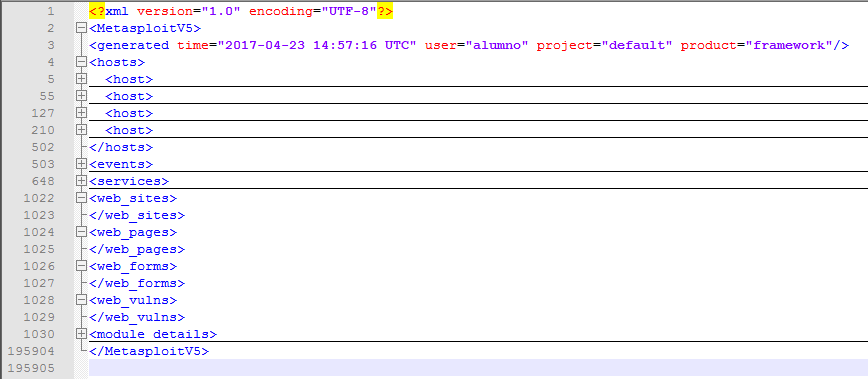
\includegraphics[width=1.0\textwidth]{./images/Atacante_scaner_y_BBDD.png}
  \caption{Atacante\_wireshar\_scaneo\_delay.}
  \label{fig:nmap6}
  \end{figure}
\end{itemize}

% #######################   Scripts NMAP   ##################################

\subsection{Scripts NMAP}
\subsubsection{Scripts /usr/share/nmap/scripts}
En la instalación de NMAP se crea el directorio \textit{/usr/share/nmap/scripts}, este directorio contiene una lista de scripts implementados por otros usuarios y que están diseñados para ser invocados desde el comando nmap. A continuación se describen algunos:
\begin{itemize}
\item \texttt{http-git.nse}: Realiza una conexión al puerto 80 de la víctima en busca de un servidor web activo, si el puerto está abierto, se intenta localizar un directorio \emph{.git}. La existencia de este directorio implica que la víctima está realizando un control de versiones, por tanto, el siguiente paso que realiza el script es la búsqueda de coincidencias en \emph{Github}, si se encuentran coincidencias (por un perfil o proyecto público), se muestran un mensaje al usuario con toda la información que se ha podido extraer de la víctima de su repositorio.
\item \texttt{smb-server-stats.nse}: Este script explota una un fallo de \emph{Samba} corriendo sobre sistemas operativos de Windows, este vulnerabilidad permite que un usuario externo pueda solicitar los datos estadísticos del servicio, recopilando así valiosa información de los archivos que se comparten.
\item \texttt{ssh2-enum-algos.nse}: Devuelve los algoritmos de cifrado y compresión que tiene implementados la víctima. Esta información puede ser muy útil para reducir considerablemente el tiempo de los ataques por fuerza bruta.
\item \texttt{dhcp-discover.nse}: Script que recopila información del servidor DHCP de la red, se imprimirá por pantalla al usuario el valor de cada uno de los campos que se obtienen del DHCP (Gateway, mácara de subred, router, nombre de dominio, etc...). Para el funcionamiento del script no es necesario consumir una dirección IP.
\end{itemize}
\subsubsection{Realización de script básico}
Se pueden crear nuevos scripts adaptados a nuestras necesidades, que automaticen tareas habituales, o repetitivas. En la siguiente url \url{http://nmap.org/book/nse-tutorial.html} se describe la estructura que debe tener el script. Para poner en práctica este apartado, a continuación, incluye el contenido de un script realizado por nosotros, las acciones que realiza son las siguientes:
\begin{itemize}
\item Comprobar si el equipo objeto tiene el puerto 80 abierto (el número de puerto se puede cambiar a la hora de ejecutar el comando)
\item En el caso de que se cumpla el paso anterior, se entiende que existe un servidor web en el equipo, por tanto, se solicita la página \textit{index.html}, dicha página se crea por defecto en los navegadores web.
\item La página web descargada se almacena en un fichero con el mismo nombre \textit{index.html}
\end{itemize}
Para ejecutar el script, se debe escribir el siguiente comando:
\begin{verbatim}
	$ nmap -p 80 <ip> --script=http-index
\end{verbatim}
\lstinputlisting[breaklines]{doc/http-index.nse}
El script contiene un control de errores, por lo que se mostrará uno de los siguientes resultados:
\begin{itemize}
	\item ''ERROR: Fallo al obtener la url index.html"
	\item ''ERROR: Fallo al crear/abrir el fichero index.html"
	\item ''index.html Obtenido correctamente!"
\end{itemize}

% #######################   COMANDO PORTSCAN   ##################################

\subsubsection{Comando Portscan}
Accedemos a la consola de Metasploit con el comando \emph{\$msfconsole}, para encontrar las modalidades existentes de Portscan, lanzamos la búsqueda con \emph{\$search portscan}, el resultado se puede ver en la figura \ref{fig:meta2}.

\begin{figure}[htbp]
\centering
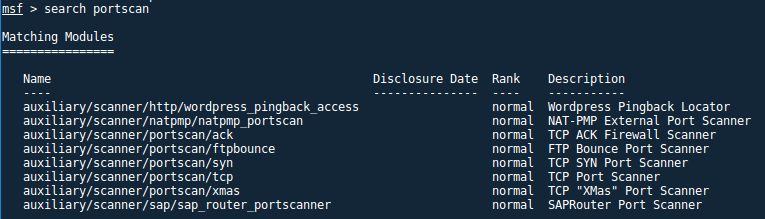
\includegraphics[width=1.0\textwidth]{./images/Atacante_metasploit_portscan_search.png}
\caption{Metasploit Portscan Search}
\label{fig:meta2}
\end{figure}

\begin{enumerate}
\item Para este ejemplo haremos uso de \emph{auxiliary/scanner/portscan/tcp}, para ello, lo seleccionamos ejecutando \emph{\$use auxiliary/scanner/portscan/tcp}.
\item Visualizamos los diferentes parámetros de configuración que permite con el comando \emph{\$show options}.
\item Ajustamos el número de hilos y la ip de la víctima.
\item Lanzamos el escaneo con el comando \emph{\$run}. Se muestra el resultado de la ejecución en la imagen \ref{fig:meta1}.
\item El funcionamiento del comando \emph{portscan} es muy similar al de Nmap, con la ventaja de poder ajustar el número de hilos que queremos dedicar al escaneo.
\end{enumerate}

\begin{figure}[htbp]
\centering
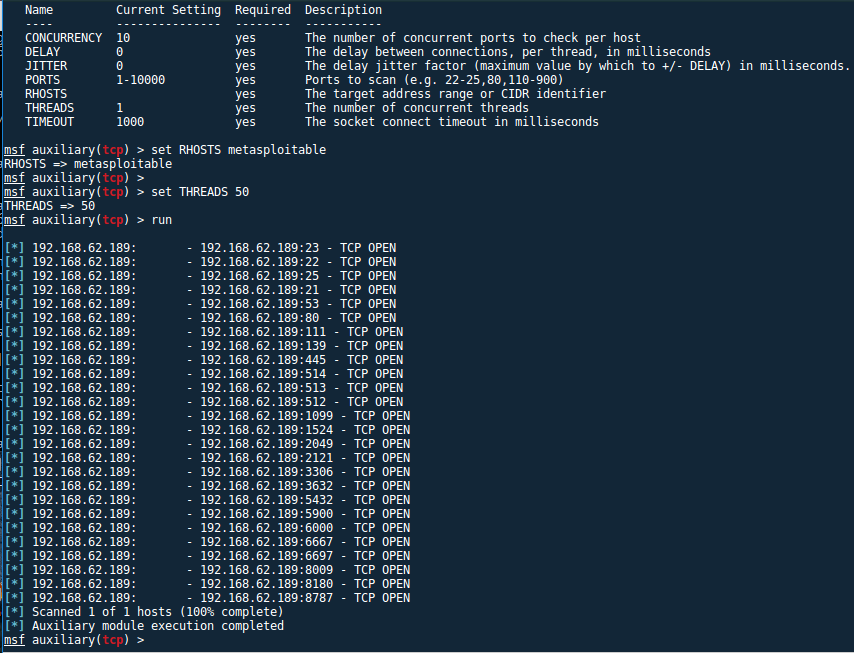
\includegraphics[width=1.0\textwidth]{./images/Atacante_metasploit_portscan.png}
\caption{Metasploit Portscan}
\label{fig:meta1}
\end{figure}

% #######################   EXPLOTAR VULNERABILIDADES   ##################################

\clearpage
\section{Explotar Vulnerabilidades}
\rhead[\thepage]{\thesection. Explotar Vulnerabilidades}

% #######################   INSTALACIÓN DE LA INTERFAZ GRÁFICA   ##################################

\subsection{Instalación de la interfaz gráfica}
Para usuarios que no son expertos en el uso de Metasploit, se recomienda el uso de la interfaz gráfica del programa, que se puede descargar desde el \href{https://www.rapid7.com/products/metasploit/download/}{siguiente enlace}. La instalación es muy simple en Linux, basta con descargarse el programa, convertirlo en ejecutable (\texttt{\$ chmod 777 metasploit-latest-linux-x64-installer.run}) y ejecutar el fichero (\texttt{.run}). Se abrirá un instalador gráfico intuitivo. \\

Para hacer uso del programa, abrimos un navegador web y accedemos a la URL que se nos indicó durante la instalación, si no hemos modificado las opciones por defecto, será \emph{https://localhost:3790/}. En la figura \ref{fig:meta3} podemos ver la apariencia.

\begin{figure}[htbp]
\centering
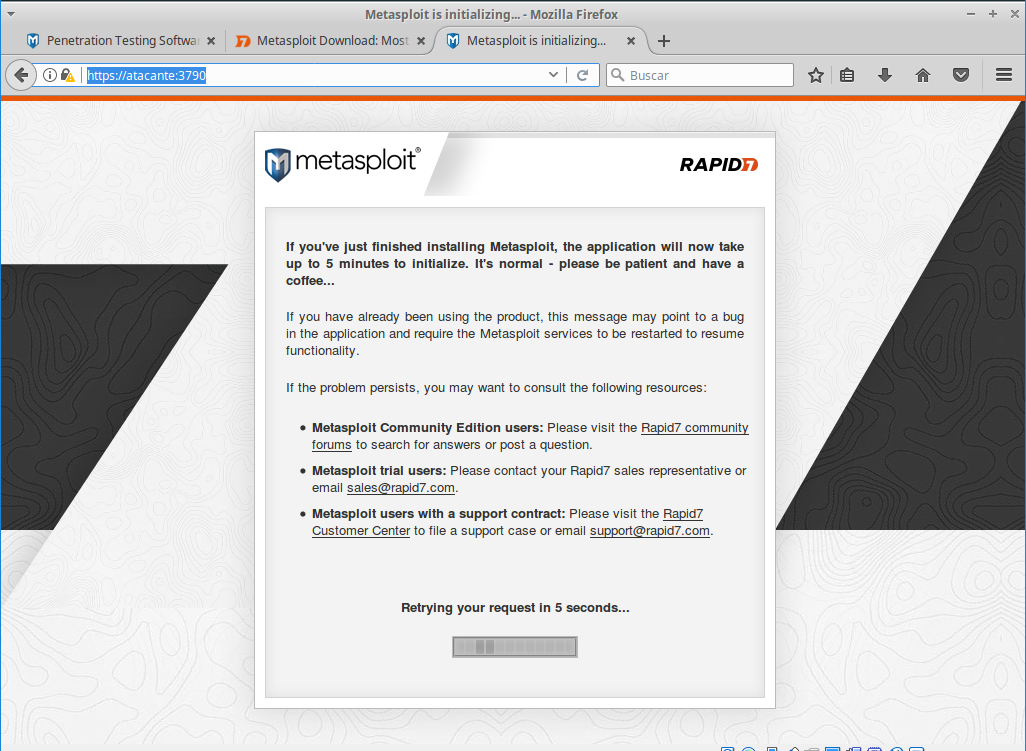
\includegraphics[width=1.0\textwidth]{./images/Atacante_metasploit_grafico.png}
\caption{Metasploit Gráfico}
\label{fig:meta3}
\end{figure}

% #######################   VNC POR FUERZA BRUTA   ##################################

\subsection{VNC por fuerza bruta}
A continuación, se muestra un ataque al servicio VNC.
\begin{itemize}
	\item Realizamos un escaneo de puertos para verificar que el de VNC está abierto. Con NMAP se ve claramente, indica el nombre de servicio.
	\begin{verbatim}
		$ sudo nmap metasploitable
	\end{verbatim}
	
	\item Accedemos a la consola de Metasploit.
		\begin{verbatim}
			$ sudo msfconsole
		\end{verbatim}
	
	\item Realizamos una búsqueda de los módulos relativos a VNC.
		\begin{verbatim}
			msf > search vnc
		\end{verbatim}
	
	\item Utilizaremos el módulo \emph{vnc\_login}, lo selecionamos.
		\begin{verbatim}
			msf > use auxiliary/scanner/vnc/vnc_login
		\end{verbatim}
	
	\item Fijamos los parámetros del ataque. Figura \ref{fig:vnc1}.

\begin{figure}[htbp]
\centering
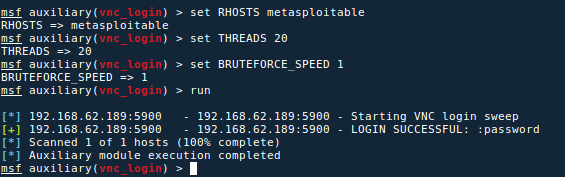
\includegraphics[width=1.0\textwidth]{./images/vnc/parametros_ataque_vnc.png}
\caption{Parámetro ataque VNC.}
\label{fig:vnc1}
\end{figure}
	
\end{itemize}

%%%%%%%%%% Snort
\clearpage
\section{Snort}
\rhead[\thepage]{\thesection. Snort}

\subsection{Configuración}

El primer paso es instalar Snort en la máquina que hace de router entre las organizaciones.

\begin{verbatim}
  $ sudo apt-get install snort
\end{verbatim}

Como vemos en la imagen \ref{fig:snort1}, el establecimiento de un rango de IPs es determinante para el uso del servicio.

\begin{figure}[htbp]
\centering
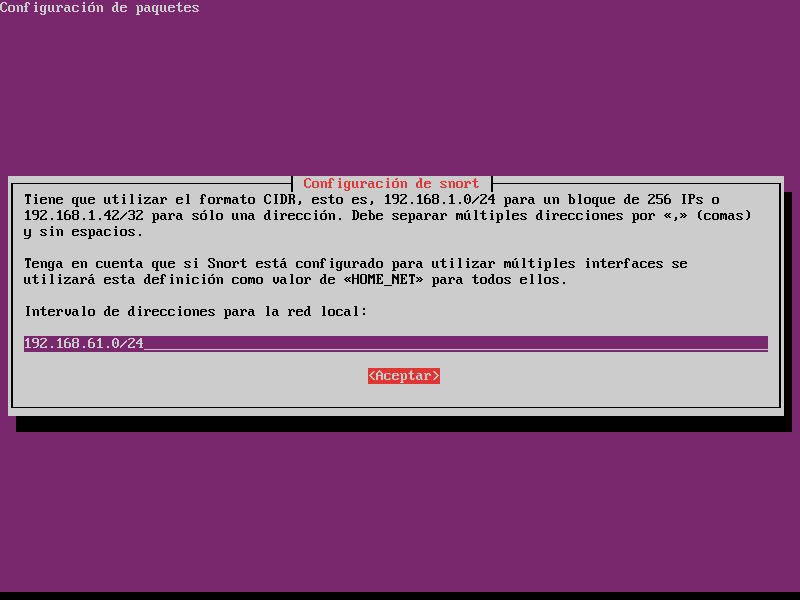
\includegraphics[width=0.9\textwidth]{./images/SnortInstalacion.jpg}
\caption{Configuración de Snort durante la instalación.}
\label{fig:snort1}
\end{figure}

A continuación se configura el servicio, modificando el fichero \emph{/etc/snort/snort.conf} y estableciendo los siguientes parámetros:

\begin{itemize}
  \item ipvar HOME\_NET 192.168.N1.0/24
  \item ipvar EXTERNAL\_NET !\$HOME\_NET
  \item ipvar DNS\_SERVERS \$HOME\_NET
  \item ipvar SMTP\_SERVERS    \$HOME\_NET
  \item ipvar HTTP\_SERVERS    \$HOME\_NET
  \item ipvar SQL\_SERVERS     \$HOME\_NET
  \item ipvar TELNET\_SERVERS  \$HOME\_NET
  \item ipvar HTTP\_PORTS      80
  \item ipvar SHELLCODE\_PORTS !80
  \item ipvar ORACLE\_PORTS    1521
\end{itemize}

\subsection{Ejecución}

Además de las reglas que hay añadidas por defecto, para poder hacer pruebas concretas y observar el funcionamiento de Snort, añadimos la siguiente línea al fichero \emph{/etc/snort/rules/local.rules}, que establece una alerta cuando detecte mensajes ICMP.

\begin{verbatim}
  $ alert icmp any any -> $HOME_NET any (msg:"ICMP test";
  sid:10000001; rev:001)
\end{verbatim}

A continuación, lanzamos el servicio. En la figura \ref{fig:snort2} se observa el servicio iniciado.

\begin{verbatim}
  $ sudo snort -i enp0s8 –u snort –g snort -l /var/log/snort/
  -A full -c /etc/snort/snort.conf
\end{verbatim}

\begin{figure}[H]
\centering
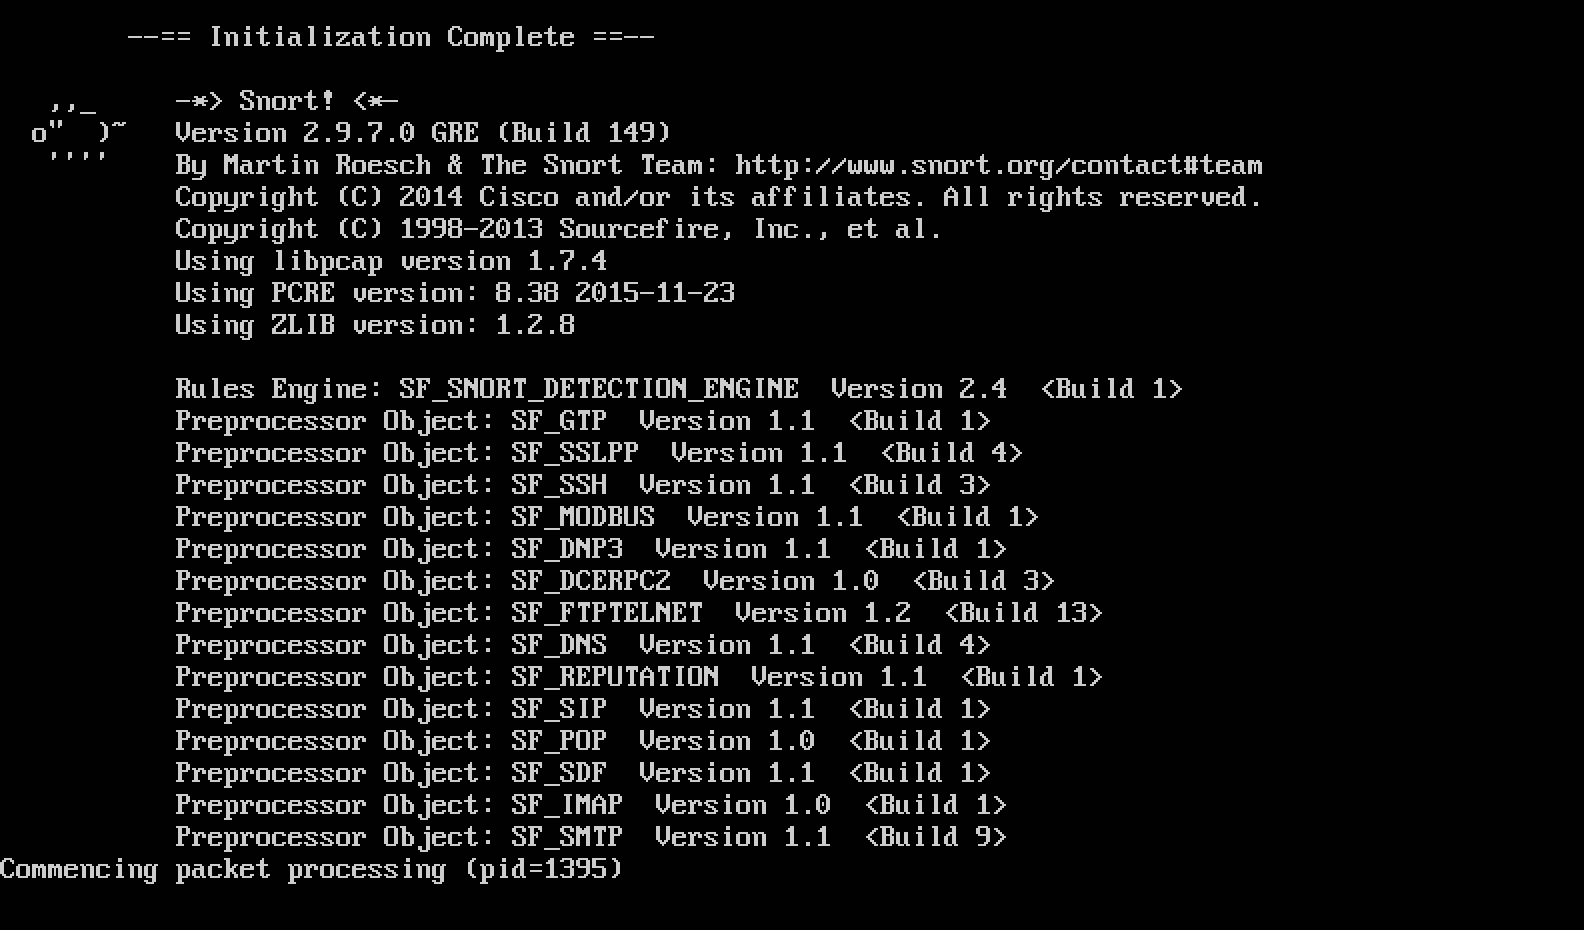
\includegraphics[width=0.9\textwidth]{./images/SnortInicio.png}
\caption{Snort iniciado.}
\label{fig:snort2}
\end{figure}

Seguidamente, lanzamos un ping desde la máquina atacante hacia la organización que el router protege, como muestra la figura \ref{fig:snort3}).

\begin{figure}[H]
\centering
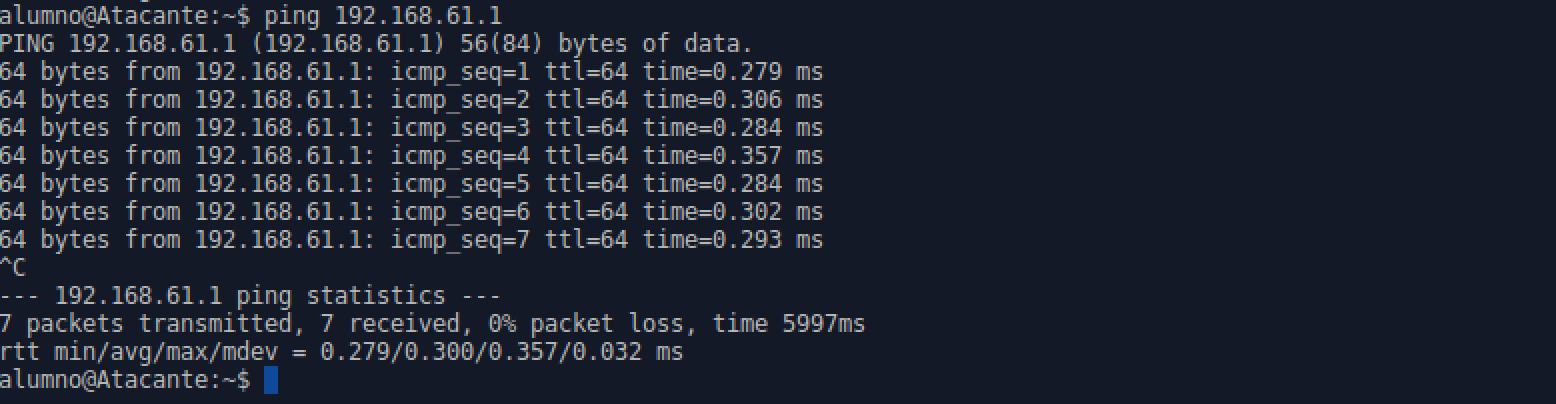
\includegraphics[width=1.0\textwidth]{./images/SnortPing.png}
\caption{Ping del atacante a la víctima.}
\label{fig:snort3}
\end{figure}

Si, tras el ping, accedemos a los archivos de log (imagen \ref{fig:snort4}), podemos ver cómo hay un acceso desde la máquina atacante.

\begin{figure}[htbp]
\centering
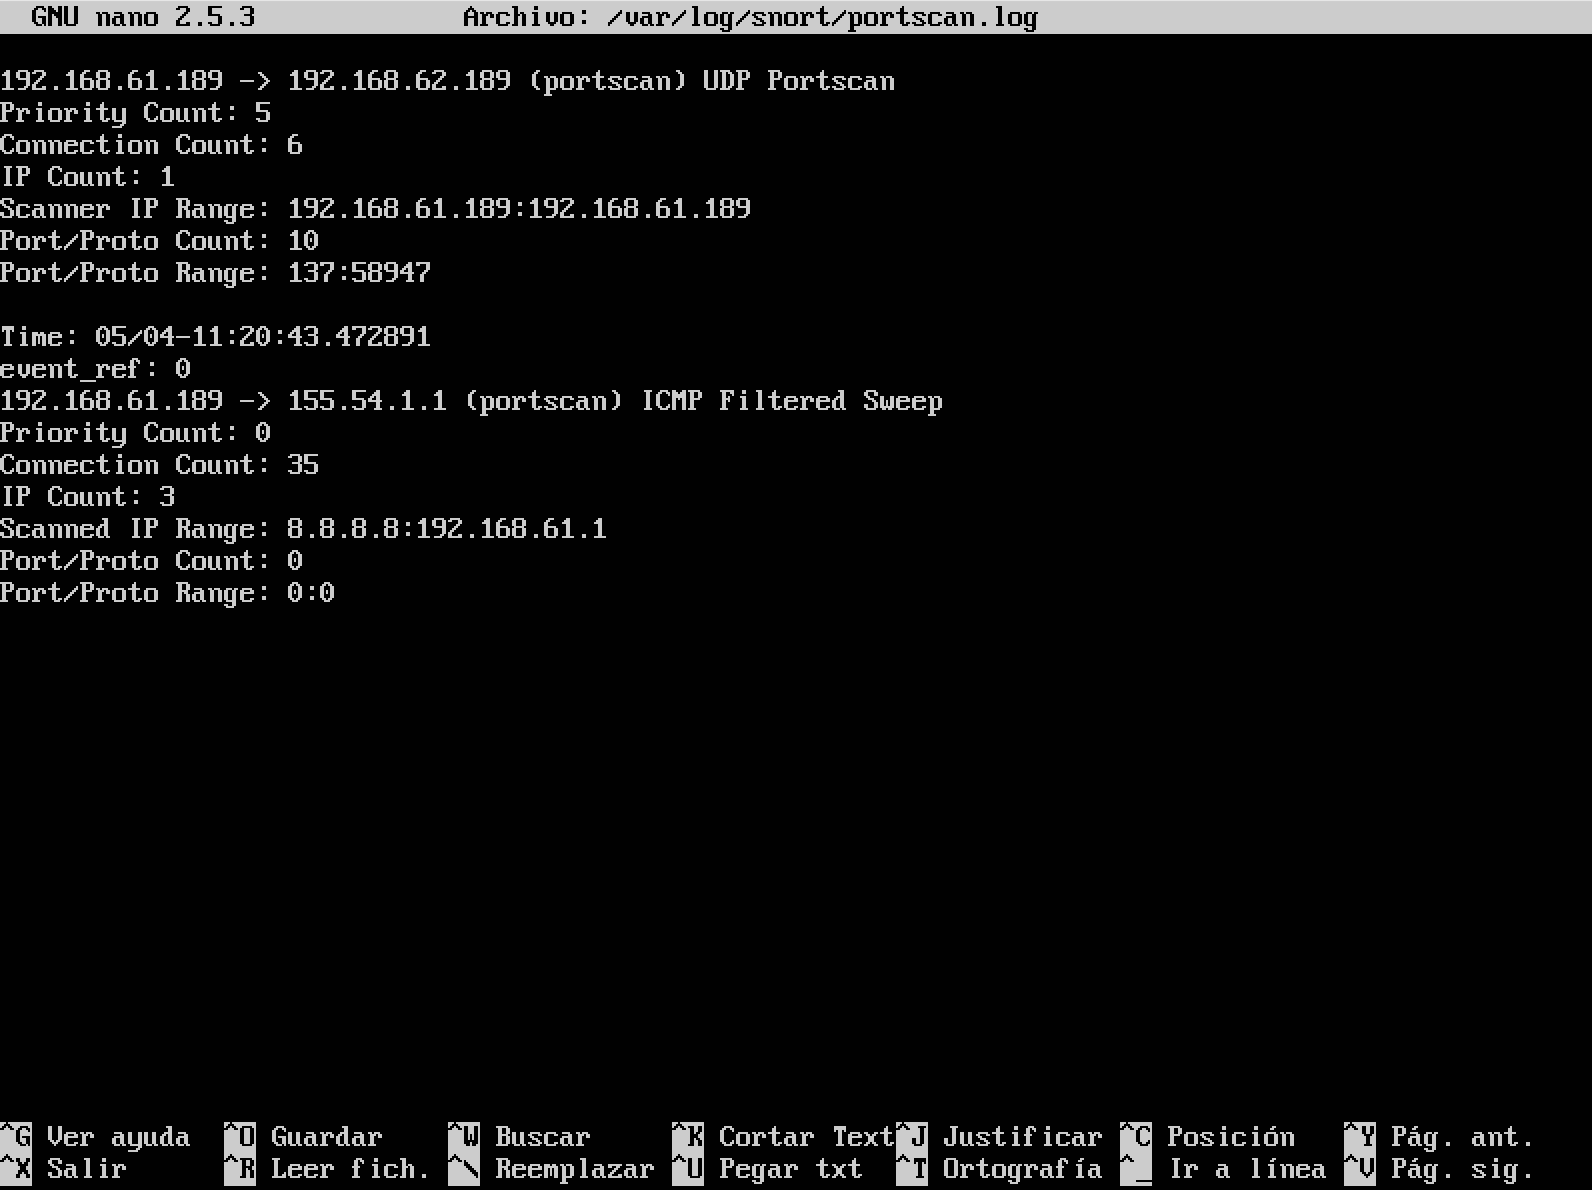
\includegraphics[width=1.0\textwidth]{./images/SnortPortLog.png}
\caption{Fichero portlog.scan tras ping.}
\label{fig:snort4}
\end{figure}

\subsection{Detección de ataques}

A continuación vamos a ejemplificar el procedimiento que el atacante sigue para llevar a cabo un ataque. Al mismo tiempo que se realiza, podemos ver los logs que detectan dicho ataque gracias a Snort.

\begin{enumerate}
  \item Escanear puertos en busca de un agujero por el que entrar. \\

  Tras ejecutar el comando nmap que se indica a continuación, se puede ver que son diversos los puertos que hay accesibles en la víctima. En este ejemplo, vamos a atacar el puerto 23, correspondiente a telnet.

  \begin{verbatim}
  $ npam -p 1-20000 192.168.62.189
  \end{verbatim}

  \begin{figure}[H]
  \centering
  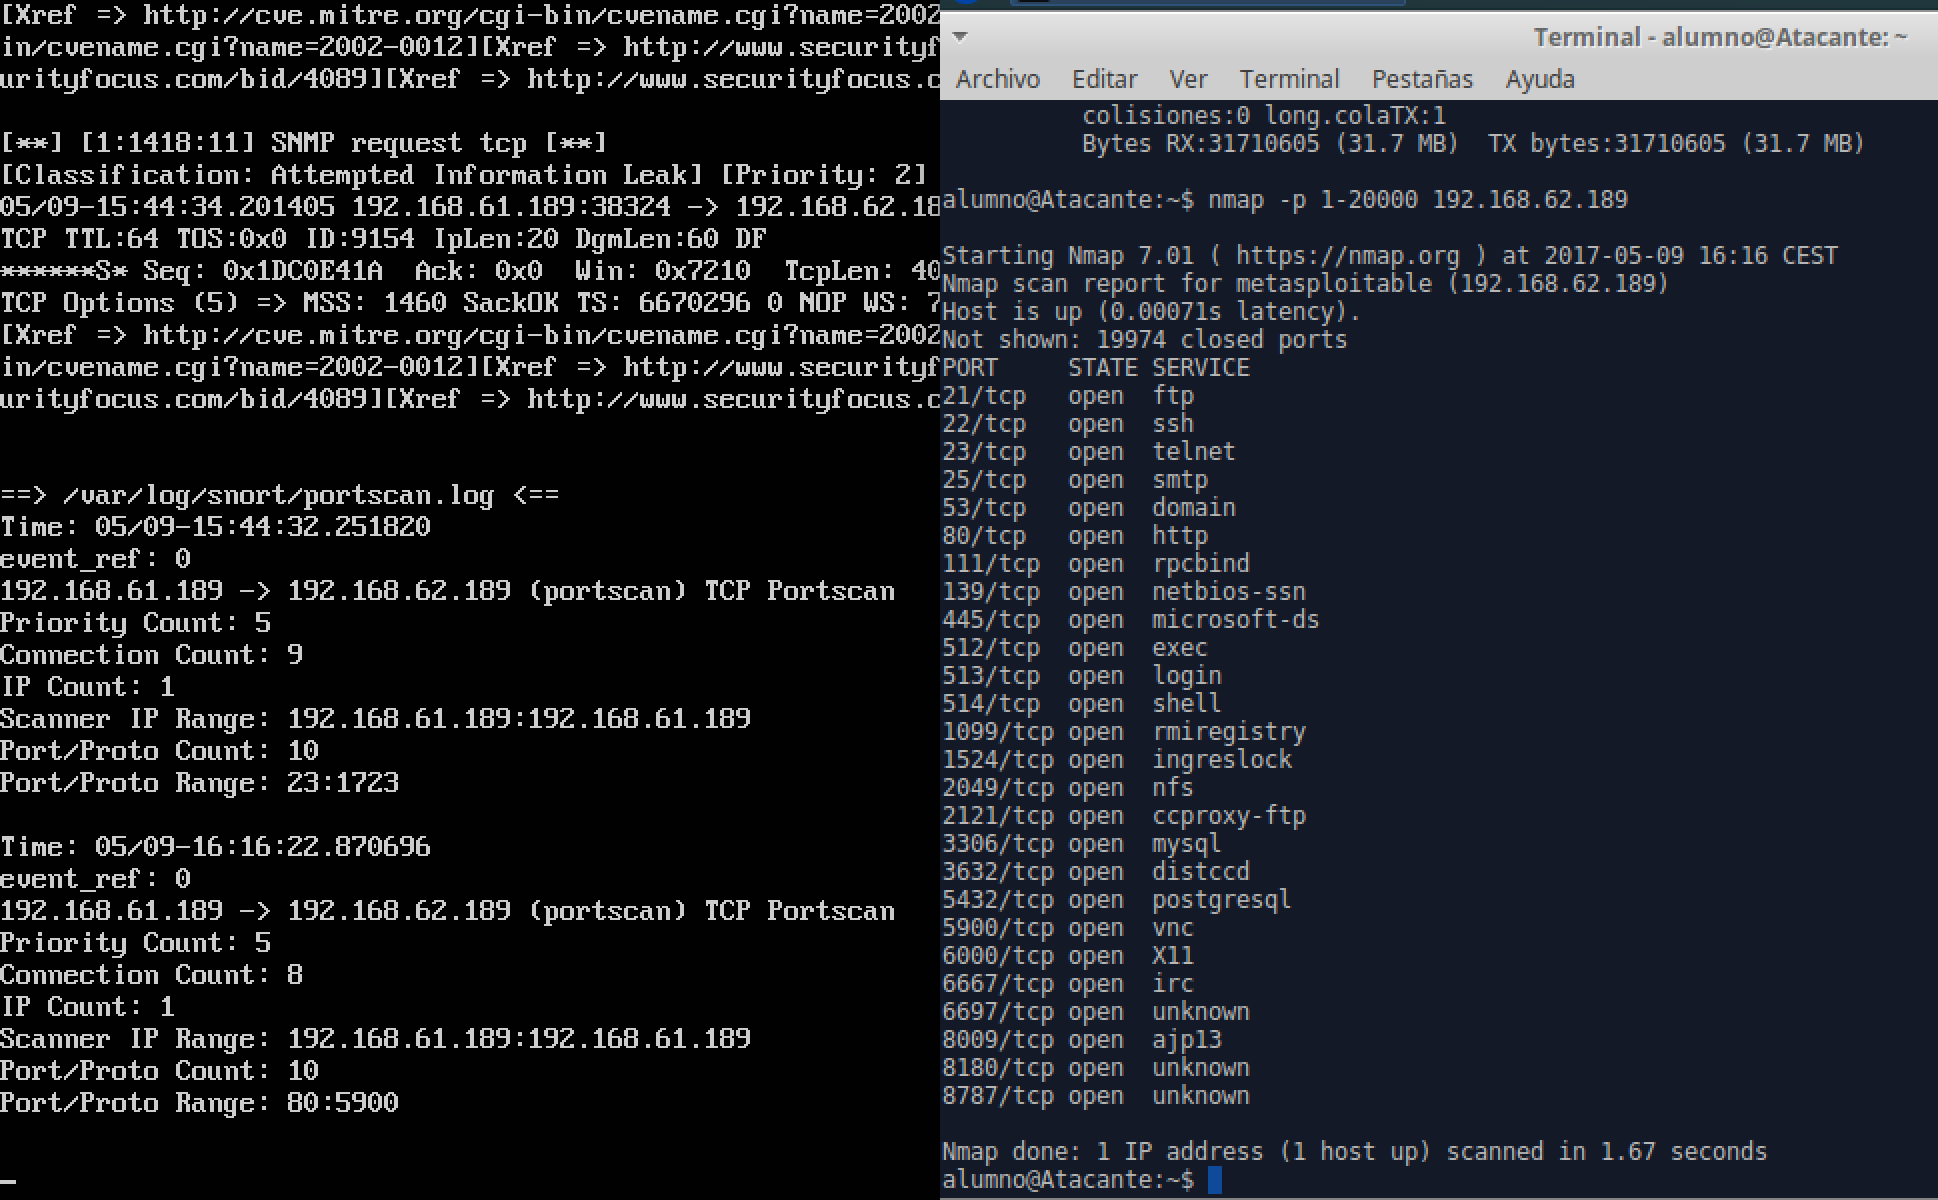
\includegraphics[width=0.8\textwidth]{./images/SnortEscaneoNmap.png}
  \caption{Escaneo nmap y logs asociados.}
  \label{fig:snort5}
  \end{figure}

  \item Acceder a la máquina en dicho puerto. \\

  Para que Snort detecte este ataque, primero debe estar configurada la detección del mismo. Para ello, añadimos en el fichero \emph{/etc/snort/snort.conf} la línea correspondiente a las reglas de telnet, como observamos en la figura \ref{fig:snort6}. \\

  Además, conviene añadir en el fichero \emph{/etc/snort/rules/local.rules} las alertas para telnet, como se ve en la figura \ref{fig:snort7}.

  \begin{figure}[H]
  \centering
  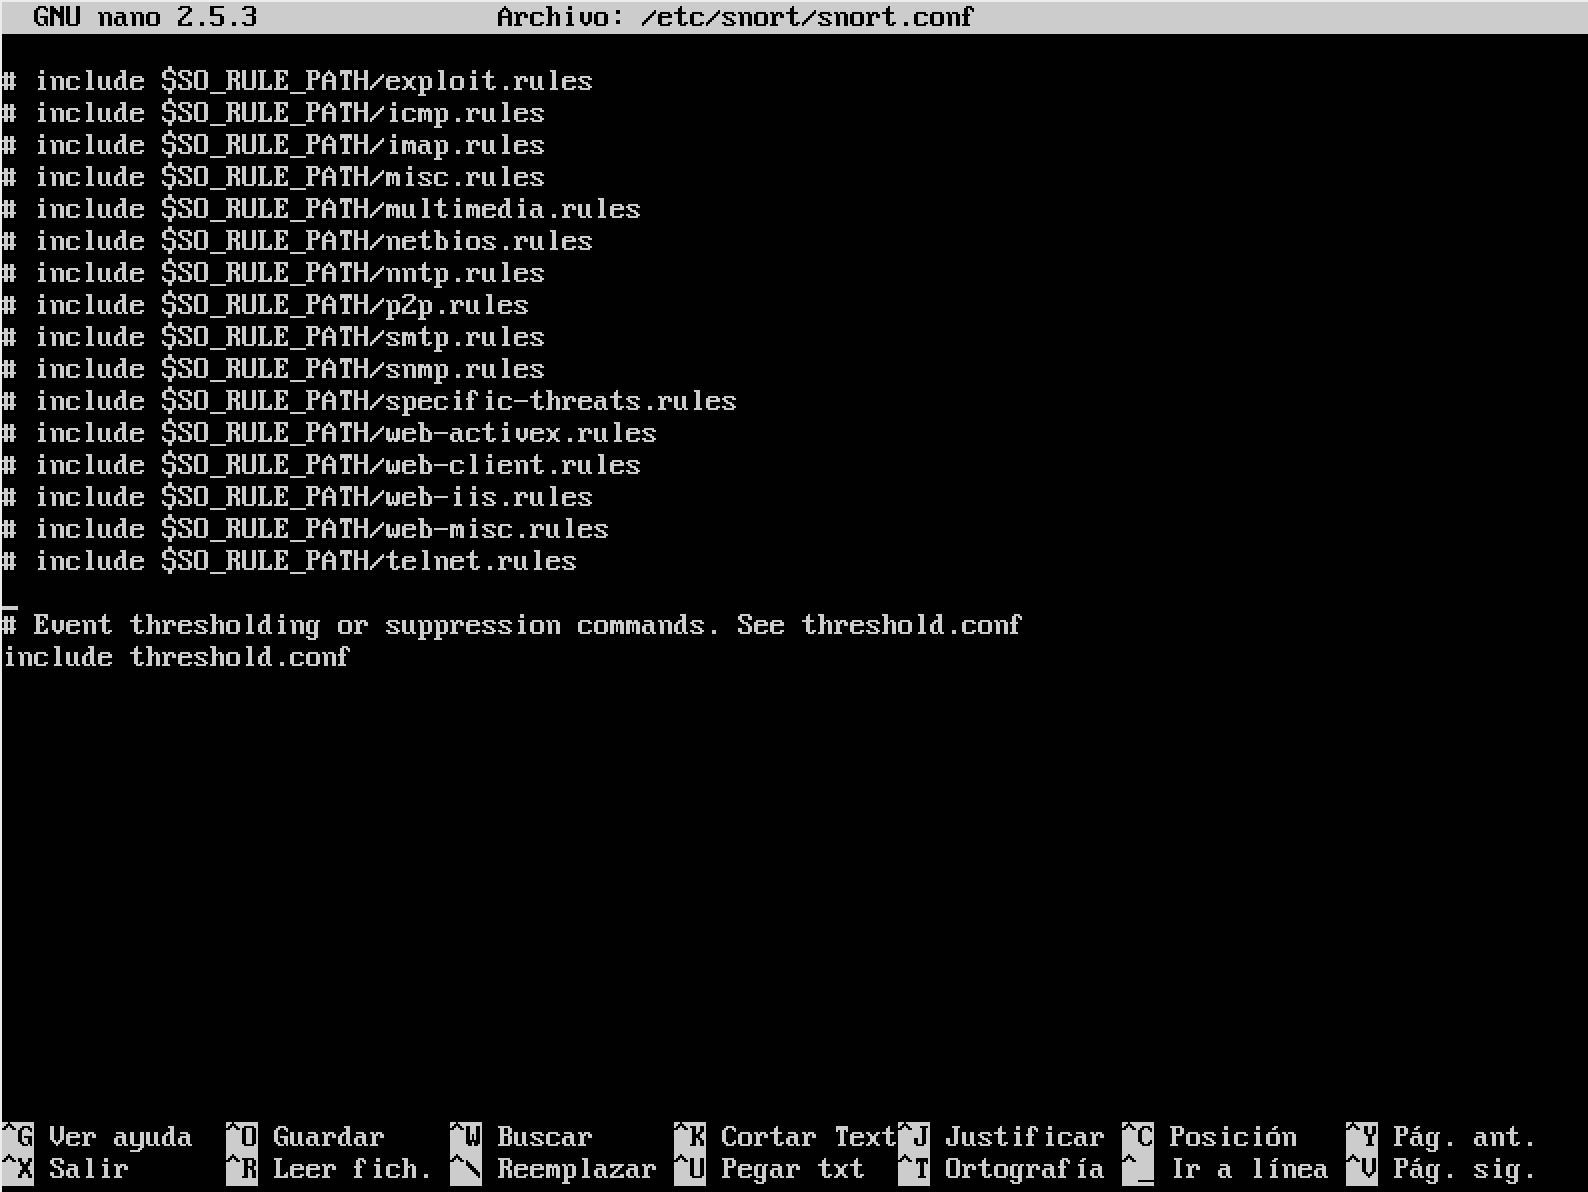
\includegraphics[width=0.8\textwidth]{./images/SnortRules.png}
  \caption{Fichero snort.conf.}
  \label{fig:snort6}
  \end{figure}

  \begin{figure}[H]
  \centering
  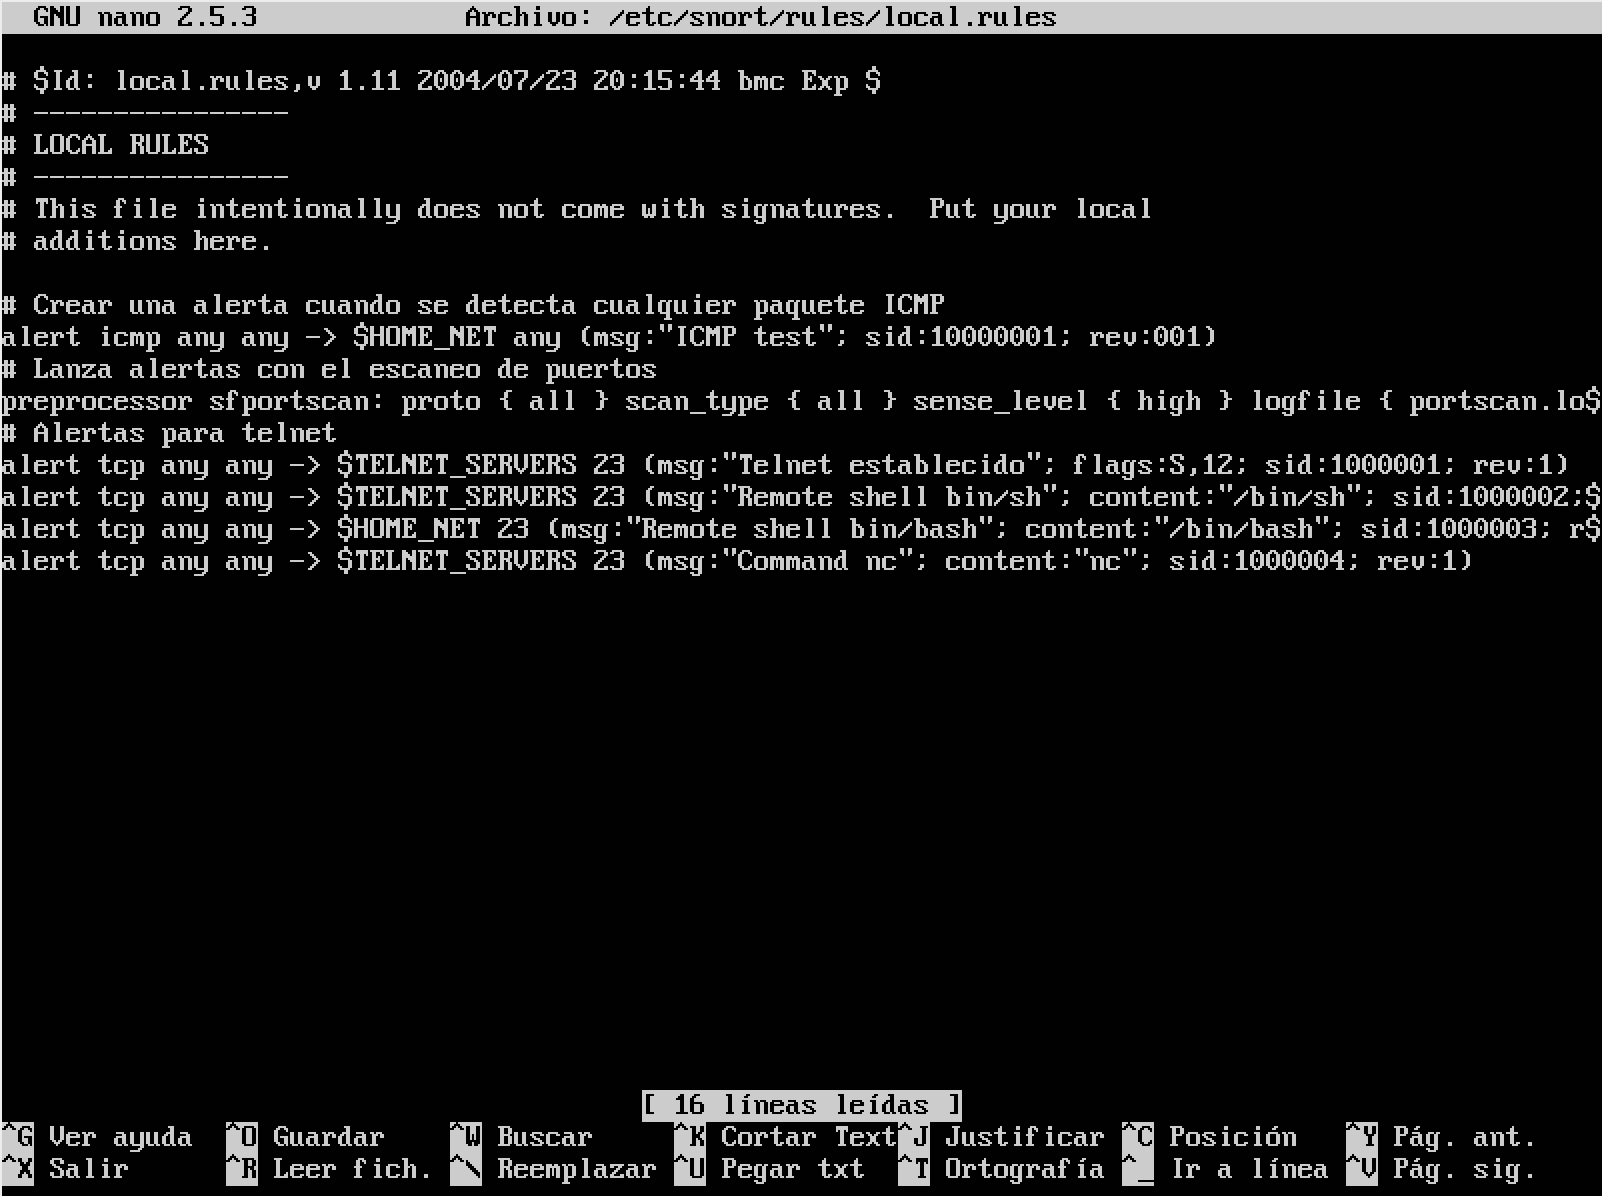
\includegraphics[width=0.8\textwidth]{./images/SnortLocal.png}
  \caption{Fichero local.rules.}
  \label{fig:snort7}
  \end{figure}

  Una vez configurado lo anterior y relanzado el servicio, procedemos a atacar el puerto con telnet, como refleja la figura \ref{fig:snort8}.

  \begin{verbatim}
   $ telnet 192.168.62.189
  \end{verbatim}

  \begin{figure}[H]
  \centering
  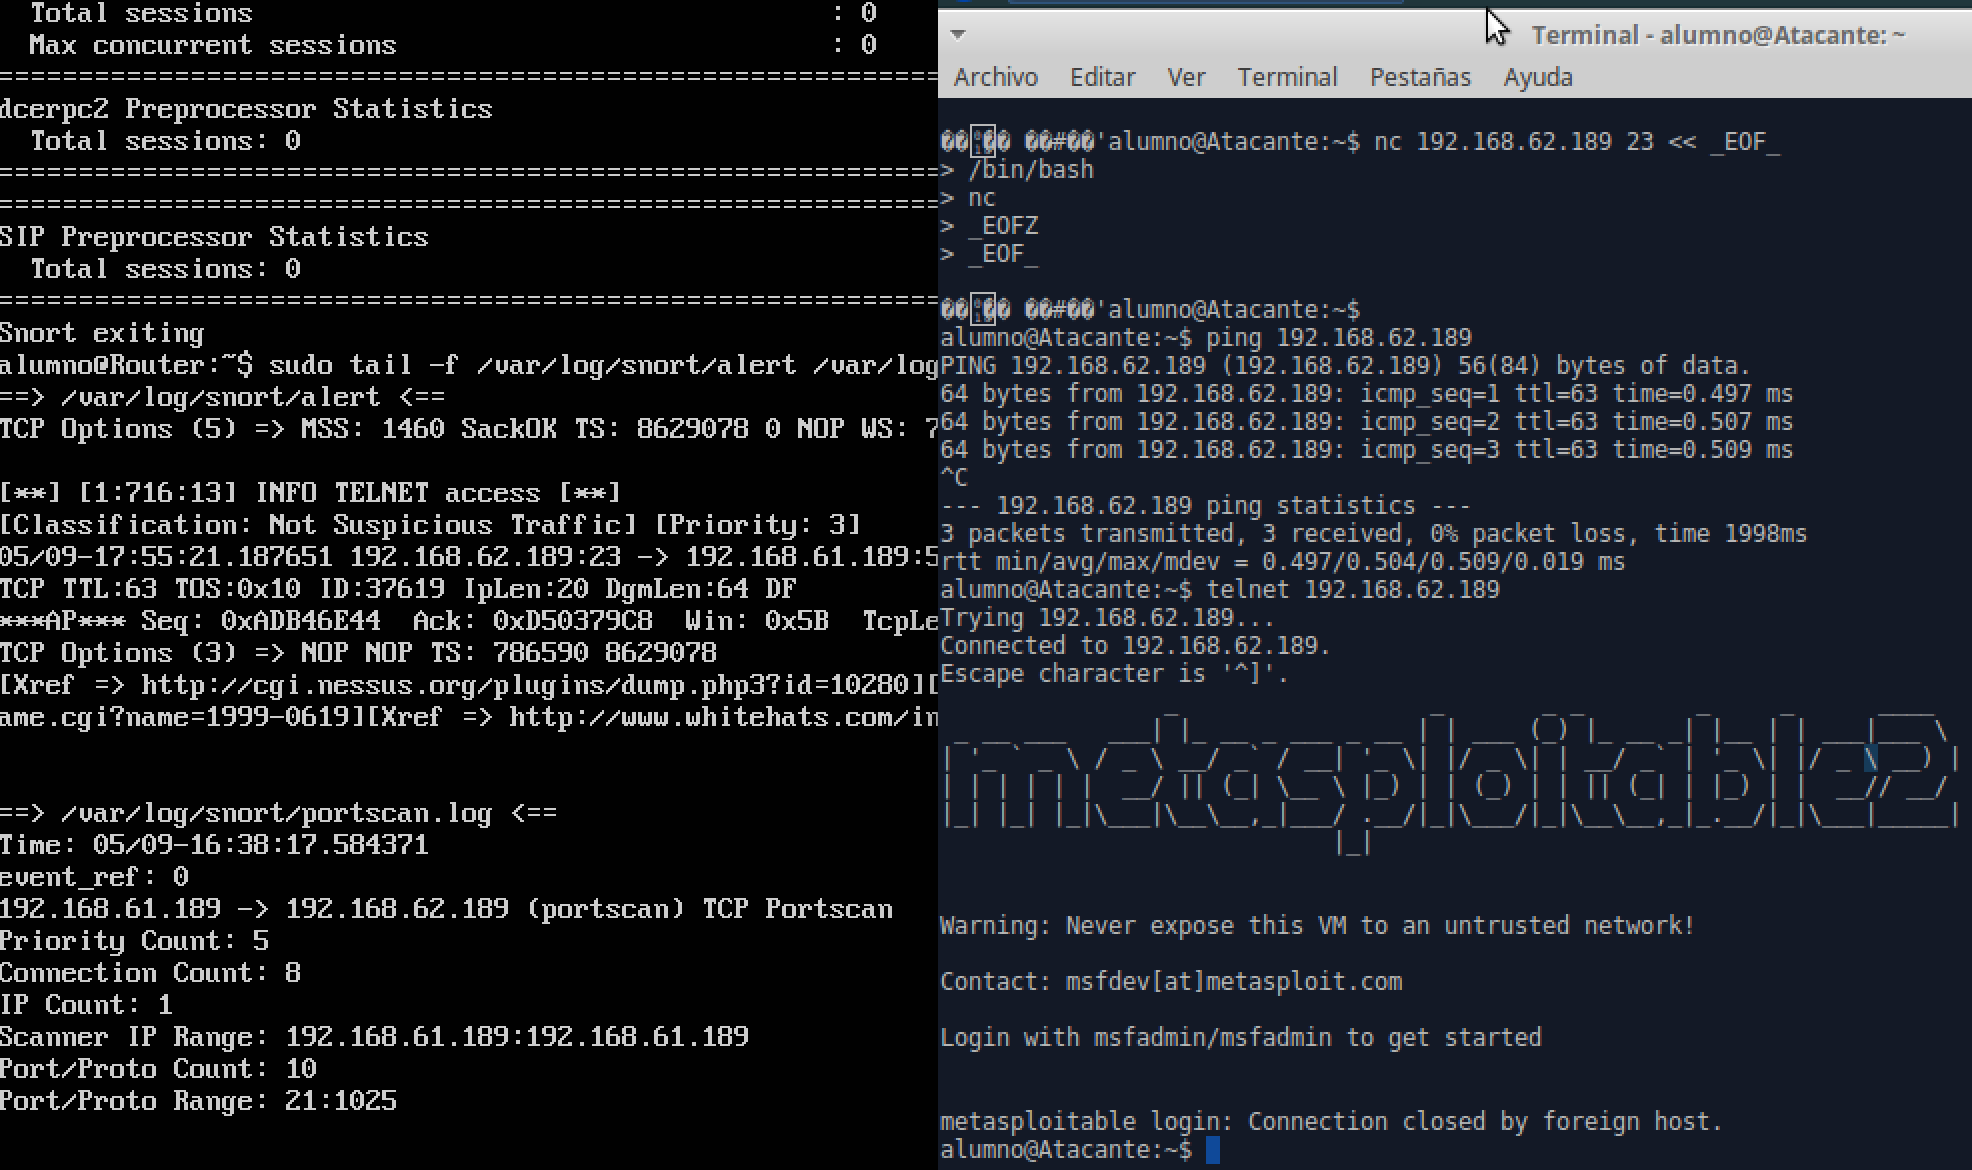
\includegraphics[width=0.8\textwidth]{./images/SnortTelnet.png}
  \caption{Comando telnet y logs asociados.}
  \label{fig:snort8}
  \end{figure}

  \item Ejecutar una orden o un shell (/bin/sh o /bin/bash) en la víctima. \\

  Una vez dentro de la víctima, podemos hacer lo que queramos. En este caso, ejecutamos un shell.

  \begin{verbatim}
   $ nc 192.168.62.189 23 << _EOF_
   > /bin/sh
   > nc
   > _EOF_
  \end{verbatim}

  En la figura \ref{fig:snort9} se pueden observar los logs generados de tal shell.

  \begin{figure}[htbp]
  \centering
  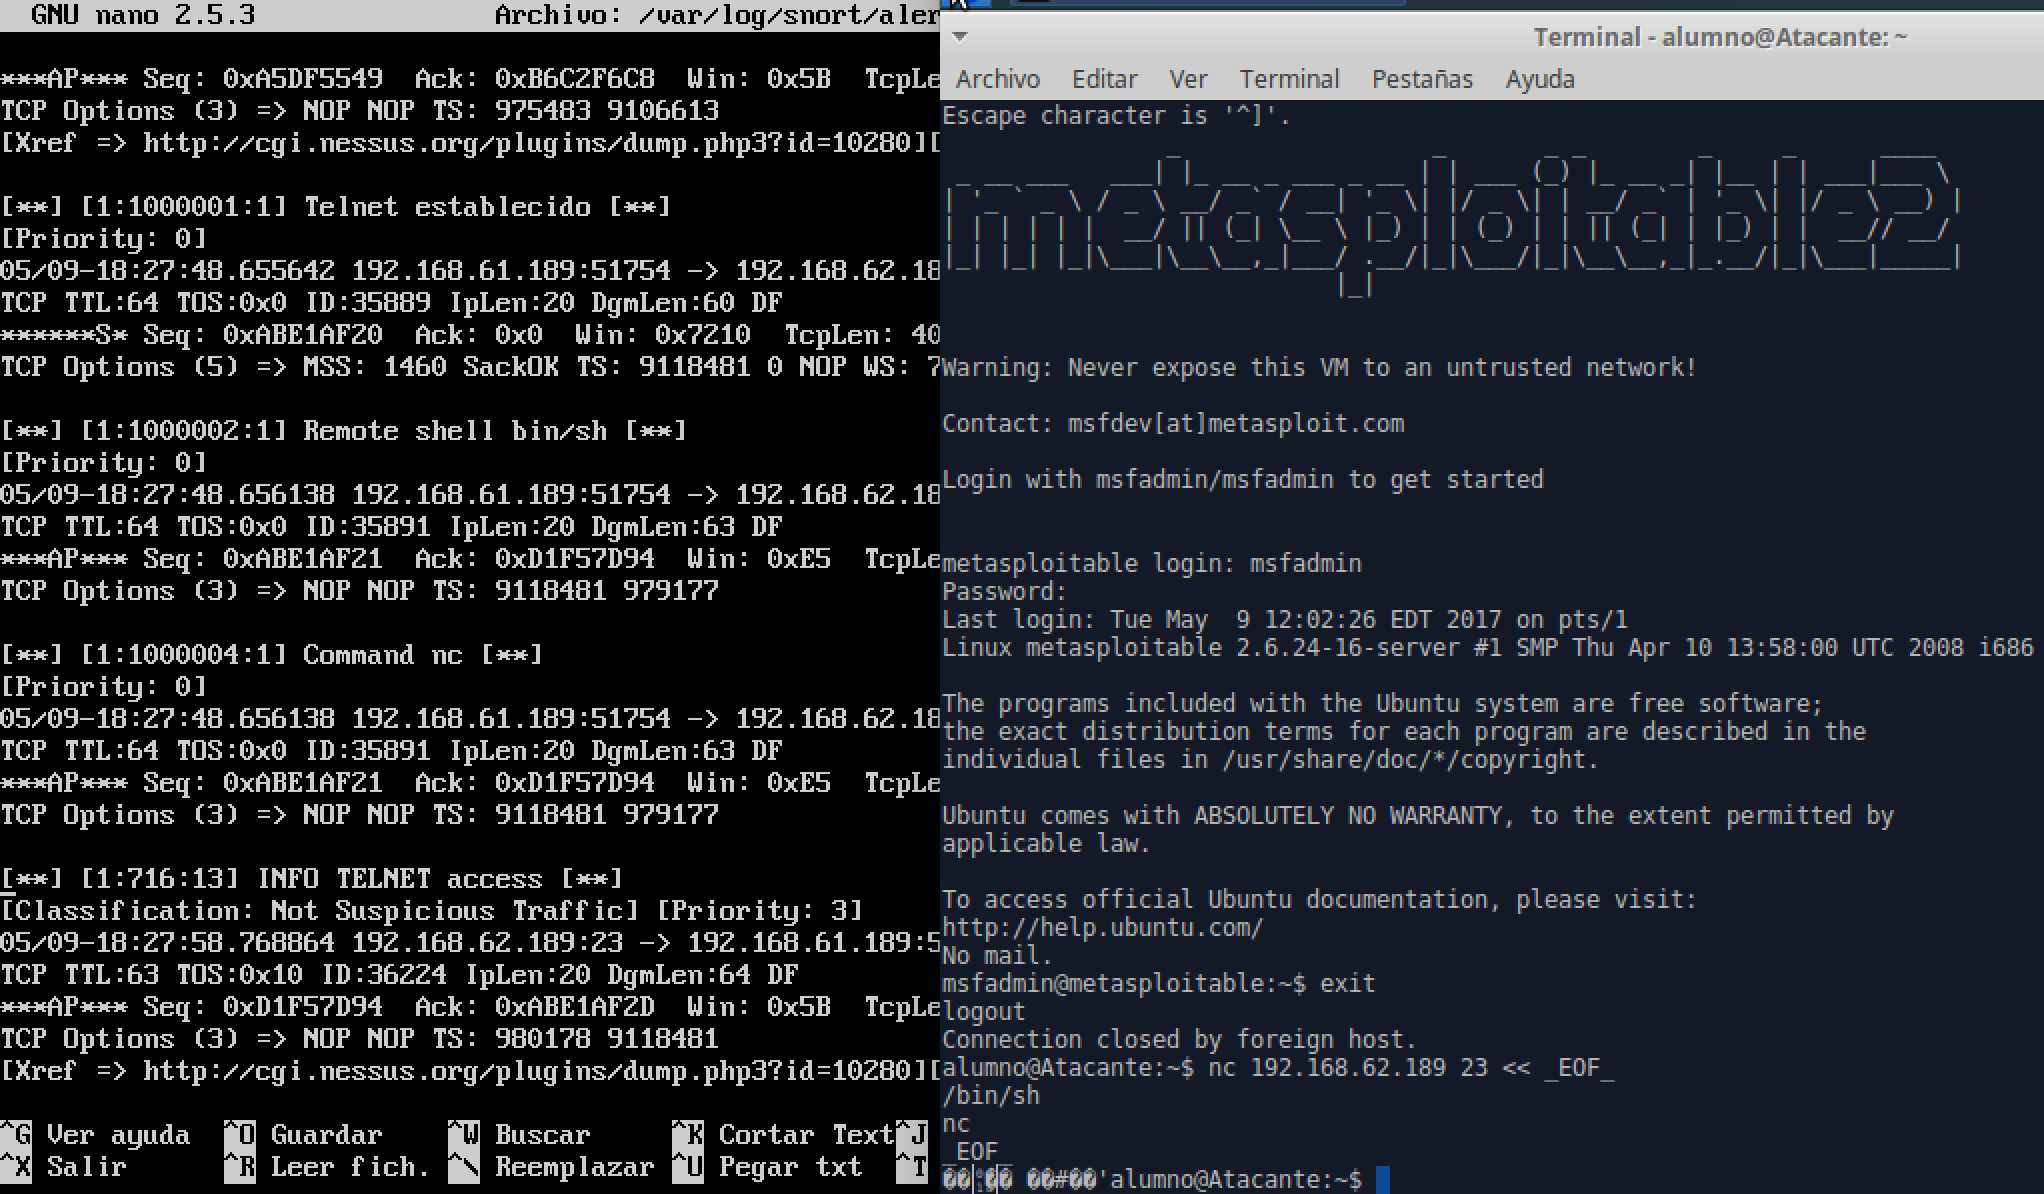
\includegraphics[width=0.9\textwidth]{./images/Snortnc.png}
  \caption{Logs generados tras nc.}
  \label{fig:snort9}
  \end{figure}

\end{enumerate}

\end{document}
